%%%%%%%%%%%%%%%%%%%%%%%%%%%%%%%%%%%%%%%%%
% Short Sectioned Assignment LaTeX Template Version 1.0 (5/5/12)
% This template has been downloaded from: http://www.LaTeXTemplates.com
% Original author:  Frits Wenneker (http://www.howtotex.com)
% License: CC BY-NC-SA 3.0 (http://creativecommons.org/licenses/by-nc-sa/3.0/)
%%%%%%%%%%%%%%%%%%%%%%%%%%%%%%%%%%%%%%%%%

%----------------------------------------------------------------------------------------
%	PACKAGES AND OTHER DOCUMENT CONFIGURATIONS
%----------------------------------------------------------------------------------------

\documentclass[paper=a4, fontsize=11pt]{scrartcl} % A4 paper and 11pt font size

% ---- Entrada y salida de texto -----

\usepackage[T1]{fontenc} % Use 8-bit encoding that has 256 glyphs
\usepackage[utf8]{inputenc}
%\usepackage{fourier} % Use the Adobe Utopia font for the document - comment this line to return to the LaTeX default

% ---- Idioma --------
\usepackage[spanish]{babel}
%\usepackage[spanish]{babel} % Selecciona el español para palabras introducidas automáticamente, p.ej. "septiembre" en la fecha y especifica que se use la palabra Tabla en vez de Cuadro

% ---- Otros paquetes ----

\usepackage{url} % ,href} %para incluir URLs e hipervínculos dentro del texto (aunque hay que instalar href)
\usepackage{amsmath,amsfonts,amsthm} % Math packages
%\usepackage{graphics,graphicx, floatrow} %para incluir imágenes y notas en las imágenes
\usepackage{graphics,graphicx, float} %para incluir imágenes y colocarlas

% Para hacer tablas comlejas
%\usepackage{multirow}
%\usepackage{threeparttable}

%\usepackage{sectsty} % Allows customizing section commands
%\allsectionsfont{\centering \normalfont\scshape} % Make all sections centered, the default font and small caps

\usepackage{fancyhdr} % Custom headers and footers
\pagestyle{fancyplain} % Makes all pages in the document conform to the custom headers and footers
\fancyhead{} % No page header - if you want one, create it in the same way as the footers below
\fancyfoot[L]{} % Empty left footer
\fancyfoot[C]{} % Empty center footer
\fancyfoot[R]{\thepage} % Page numbering for right footer
\renewcommand{\headrulewidth}{0pt} % Remove header underlines
\renewcommand{\footrulewidth}{0pt} % Remove footer underlines
\setlength{\headheight}{13.6pt} % Customize the height of the header

\numberwithin{equation}{section} % Number equations within sections (i.e. 1.1, 1.2, 2.1, 2.2 instead of 1, 2, 3, 4)
\numberwithin{figure}{section} % Number figures within sections (i.e. 1.1, 1.2, 2.1, 2.2 instead of 1, 2, 3, 4)
\numberwithin{table}{section} % Number tables within sections (i.e. 1.1, 1.2, 2.1, 2.2 instead of 1, 2, 3, 4)

\setlength\parindent{0pt} % Removes all indentation from paragraphs - comment this line for an assignment with lots of text

\newcommand{\horrule}[1]{\rule{\linewidth}{#1}} % Create horizontal rule command with 1 argument of height

\graphicspath{ {./images/} }
\usepackage{subcaption}
\usepackage{hyperref}
\usepackage{soul}


%----------------------------------------------------------------------------------------
%	TÍTULO Y DATOS DEL ALUMNO
%----------------------------------------------------------------------------------------

\title{	
\normalfont \normalsize 
\textsc{\textbf{Introducción a la Ciencia de Datos (2019)} \\ Máster Oficial Universitario en Ciencia de Datos e Ingeniería de Computadores \\ Universidad de Granada} \\ [25pt] % Your university, school and/or department name(s)
\horrule{0.5pt} \\[0.4cm] % Thin top horizontal rule
\huge Trabajo Integrador: EDA, Clasificación y Regresión \\ % The assignment title
\horrule{2pt} \\[0.5cm] % Thick bottom horizontal rule
}

\author{Luis Balderas Ruiz \\ \texttt{luisbalderas@correo.ugr.es}} 
 % Nombre y apellidos 


\date{\normalsize\today} % Incluye la fecha actual

%----------------------------------------------------------------------------------------
% DOCUMENTO
%----------------------------------------------------------------------------------------

\begin{document}

\maketitle % Muestra el Título

\newpage %inserta un salto de página

\tableofcontents % para generar el índice de contenidos

\listoffigures

\listoftables

\newpage

%
%\begin{figure}[H] %con el [H] le obligamos a situar aquí la figura
%	\centering
%	\includegraphics[scale=0.6]{e1.png}  %el parámetro scale permite agrandar o achicar la imagen. En el nombre de archivo puede especificar directorios
%	\caption{Progresión de la imagen de E en cada iteración} 
%	\label{fig:e1}
%\end{figure}


%----------------------------------------------------------------------------------------
%	Introducción
%----------------------------------------------------------------------------------------

\section{Introducción}


El presente documento contiene los resultados obtenidos en el Trabajo Teórico/Práctico Integrador para la evaluación de la asignatura Introducción a la Ciencia de Datos. El trabajo está formado por tres apartados, a saber, análisis de datos (en adelante EDA), regresión y clasificación, centrado en dos conjuntos de datos: Wankara para regresión y Vowel para clasificación. Ambos dos forman parte del repositorio de Keel (\cite{keel}), el primero en \cite{wankara} y el segundo en \cite{vowel}. A continuación, describo la estructura del documento. En la primera sección, se desarrolla el análisis exploratorio de ambos datasets. A continuación, tras sacar las conclusiones correspondientes, ataco el problema de regresión y, por último, el de clasificación.






%----------------------------------------------------------------------------------------
%	Análisis de datos
%----------------------------------------------------------------------------------------

\section{Análisis exploratorio de datos (EDA)}

\subsection{Conjunto de datos Wankara}

\subsection{Conjunto de datos Vowel}

El presente conjunto de datos contiene información sobre el reconocimiento de las once vocales existentes en inglés por parte de 15 interlocutores independientes. Es un problema de clasificación de once clases (las once vocales inglesas) con trece características, diez de ellas reales y tres enteras. A pesar de ser numéricas, esas tres variables son realmente categóricas, dado que

\begin{itemize}
	\item TT (0/1): Indica si la instancia es de entrenamiento (0) o test (1).
	\item Sex (0/1): Indica el género del hablante en dicha instancia.
	\item SpeakerNumber [0,14]: Indica el interlocutor de la instancia.
\end{itemize}

\begin{figure}[H] %con el [H] le obligamos a situar aquí la figura
	\centering
	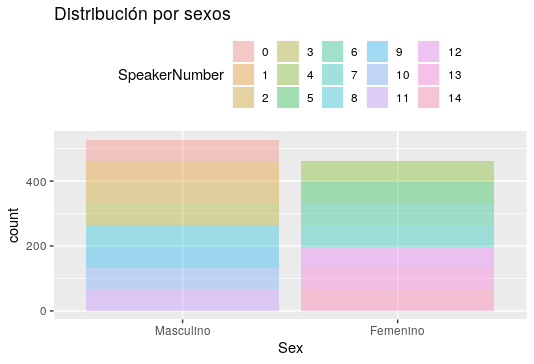
\includegraphics[scale=0.7]{dist-sexos.png}  %el parámetro scale permite agrandar o chicar la imagen. En el nombre de archivo puede especificar directorios
	\caption{Distribución por sexos de los interlocutores} 
	\label{fig:dist-sex}
\end{figure}

Por tanto, esas variables se pueden interpretar como factores más que numéricas. De hecho, TT será ignorada en el EDA porque es conveniente realizar el estudio sobre los datos al completo. Por tanto, tras estas modificaciones contamos con diez variables reales (F0-F9), dos factores (sexo y número de interlocutor) y once clases (0-10), con un total de 990 instancias. 

Para explorar los datos, en primer lugar, calculo un resumen estadístico de cada variable y su dispersión. En las variables categóricas encontramos:

\begin{itemize}
	\item Cada interlocutor tiene 66 apariciones en el conjunto de datos.
	\item 528 de ellos son hombres y 462 mujeres.
\end{itemize}

Para las variables numéricas, los resultados son los siguientes:

\begin{table}[H]
	\resizebox{\textwidth}{!}{\begin{tabular}{|c|c|c|c|c|c|c|c|c|c|c|}
		\hline
		& \textbf{F0} & \textbf{F1} & \textbf{F2} & \textbf{F3} & \textbf{F4} & \textbf{F5} & \textbf{F6} & \textbf{F7} & \textbf{F8} & \textbf{F9} \\ \hline
		\textbf{Min}     & -5.211      & -1.274      & -2.487      & -1.409      & -2.127      & -0.836      & -1.537      & -1.293      & -1.631      & -1.68       \\ \hline
		\textbf{1st Qua} & -3.888      & 1.052       & -0.97575    & -0.0655     & -0.769      & 0.196       & -0.307      & -0.09575    & -0.704      & -0.548      \\ \hline
		\textbf{Mediana} & -3.146      & 1877        & -0.5725     & 0.4335      & -0.299      & 0.552       & 0.022       & 0.328       & -0.3025     & -0.1565     \\ \hline
		\textbf{Media}   & -3.204      & 1.882       & -0.50777    & 0.5155      & -0.3057     & 0.6302      & -0.004365   & 0.33655     & -0.30298    & -0.07134    \\ \hline
		\textbf{3th Qua} & -2.603      & 2.738       & -0.06875    & 1.096       & 0.1695      & 1.0285      & 0.2965      & 0.77        & 0.09375     & 0.371       \\ \hline
		\textbf{Max}     & -0.941      & 5.074       & 1.431       & 2.377       & 1.831       & 2.327       & 1.403       & 2.039       & 1.309       & 1.396       \\ \hline
		\textbf{SD}      & 0.8689872   & 1.1752720   & 0.7119483   & 0.7592613   & 0.6646023   & 0.6038711   & 0.4619268   & 0.5733020   & 0.5701616   & 0.6039855   \\ \hline
	\end{tabular}}
	\caption{Resumen estadístico y desviación típica de las características reales}
\end{table}

Como se puede observar, el rango y el dominio de cada variable es distinto, lo que podría condicionar el rendimiento de los posteriores algoritmos que utilizaremos. Por tanto, será necesario un reescalado de las mismas para evitar esa discriminación positiva de unas variables respecto a otras sólo por ser "mayores". \\

A continuación, presento las 10 variables numéricas con más detenimiento. Una de las características principales de este conjunto de datos es que, si se estudia como un todo, el comportamiento de las variables a veces puede parecer errático. Sin embargo, no se debe soslayar el hecho de que tenemos una variable categórica, la del sexo, que nos hace prácticamente crear dos conjuntos de datos cuasi-independientes: hombres y mujeres, donde sí que encontramos correlaciones y claves para entender el funcionamiento de las características. Como digo, presento cada una de las variables, primero estudiándola en conjunto y luego separando por sexo. Para comprobar si las variables siguen una distribución normal, se han utilizado el test de Shapiro-Wilk (\cite{10.1093/biomet/52.3-4.591}) y la corrección de Lilliefors del test de Kolmogorov-Smirnov (\cite{10.1080/01621459.1967.10482916}). Además, para estudiar el comportamiento tanto por sexo como por interlocutor, represento vía boxplots cada variable.
\newpage

\subsubsection{F0}

Presentamos la variable F0. En primer lugar, reflejo un resumen estadístico de la misma así como su histograma diferenciando entre hombres y mujeres.
\begin{itemize}
	\item Media: -3.204
	\item Mediana: -3.146
	\item Desviación típica: 0.8689872
	\item Rango: [-5.211,-0.941]
	\item Primer y tercer cuartiles: (-3.888,-2.603)
	\item Asimetría: 0.0662973
	\item Curtosis: -0.4974651
\end{itemize}

Por el valor de la curtosis, la variable es platicúrtica y muy ligeramente asimétrica por la derecha.

\begin{figure}[H] %con el [H] le obligamos a situar aquí la figura
	\centering
	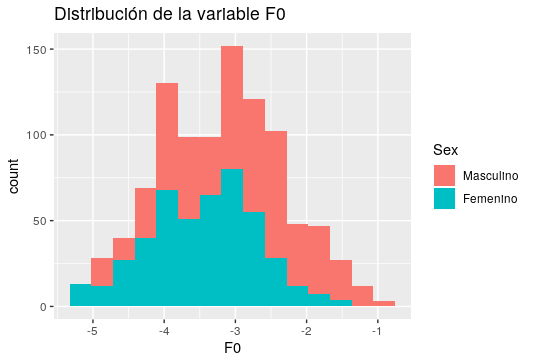
\includegraphics[scale=0.6]{dist-F0.png}  %el parámetro scale permite agrandar o chicar la imagen. En el nombre de archivo puede especificar directorios
	\caption{Histograma de la variable F0} 
	\label{fig:hist-F0}
\end{figure}

Pasamos a comprobar si F0 se distribuye según una normal. Para ello, establecemos los tests de hipótesis de Shapiro-Wilk y Lilliefors (Kolmogorov-Smirnov) con los siguientes resultados:

\begin{figure}[H]
	\centering
	\begin{subfigure}{.5\textwidth}
		\centering
		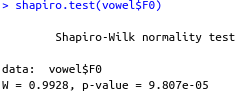
\includegraphics[width=.7\linewidth]{sw-F0.png}
		\caption{Shapiro-Wilk}
		\label{fig:sw-F0}
	\end{subfigure}%
	\begin{subfigure}{.5\textwidth}
		\centering
		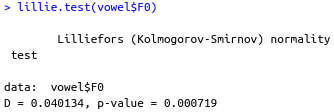
\includegraphics[width=.7\linewidth]{l-F0.png}
		\caption{Lilliefors}
		\label{fig:l-F0}
	\end{subfigure}
	\caption{Tests de normalidad sobre F0}
	\label{fig:normF0}
\end{figure}

Como los p-valores son menores que 0.05, rechazamos la hipótesis nula (la variable sigue una distribución normal). \\


A continuación presento los boxplots:

\begin{figure}[H]
	\centering
	\begin{subfigure}{.5\textwidth}
		\centering
		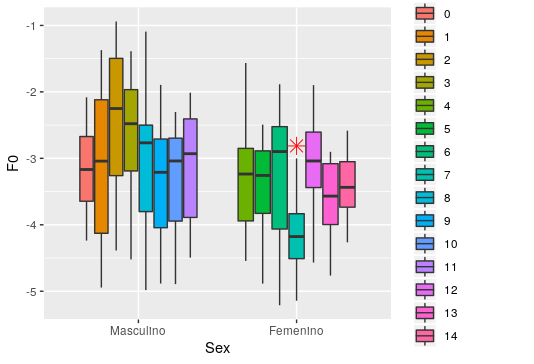
\includegraphics[width=.9\linewidth]{bps0.png}
		\caption{Por sexo}
		\label{fig:bps0}
	\end{subfigure}%
	\begin{subfigure}{.5\textwidth}
		\centering
		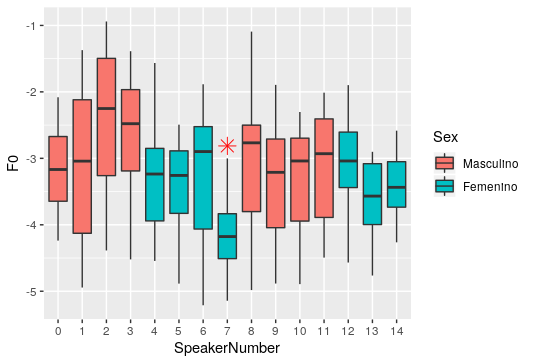
\includegraphics[width=.9\linewidth]{bpsn0.png}
		\caption{Por interlocutor}
		\label{fig:bpsn0}
	\end{subfigure}
	\caption{Boxplot para F0 estudiando sexos e interlocutores}
	\label{fig:bf0}
\end{figure}

Como se puede ver, existe un outlier en el interlocutor 7. Además, observamos que los valores para los hombres tienden a ser mayores que para las mujeres. \\

Si ahora estudiamos los tests de normalidad por sexos, encontramos los siguientes resultados:

\begin{figure}[H]
	\centering
	\begin{subfigure}{.5\textwidth}
		\centering
		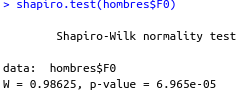
\includegraphics[width=.6\linewidth]{swh-F0.png}
		\caption{Shapiro-Wilk}
		\label{fig:swh-F0}
	\end{subfigure}%
	\begin{subfigure}{.5\textwidth}
		\centering
		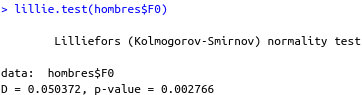
\includegraphics[width=.6\linewidth]{lh-F0.png}
		\caption{Lilliefors}
		\label{fig:lh-F0}
	\end{subfigure}
	\caption{Tests de normalidad sobre F0 (hombres)}
	\label{fig:normhF0}
\end{figure}

En este caso, aunque también se rechaza la hipótesis de normalidad, el test de Lilliefors arroja un resultado menor pero cercano a 0.05, por lo que parece acercarse más la variable en los hombres a una distribución normal que con el conjunto completo. \\

Para las mujeres,

\begin{figure}[H]
	\centering
	\begin{subfigure}{.5\textwidth}
		\centering
		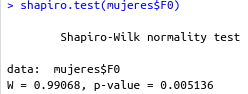
\includegraphics[width=.6\linewidth]{swm-F0.png}
		\caption{Shapiro-Wilk}
		\label{fig:swm-F0}
	\end{subfigure}%
	\begin{subfigure}{.5\textwidth}
		\centering
		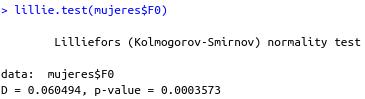
\includegraphics[width=.6\linewidth]{lm-F0.png}
		\caption{Lilliefors}
		\label{fig:lm-F0}
	\end{subfigure}
	\caption{Tests de normalidad sobre F0 (mujeres)}
	\label{fig:normmF0}
\end{figure}

se encuentran unos p-valores menores que para los hombres, por lo que también se rechaza la hipótesis de normalidad.

\subsubsection{F1}

Como en el apartado anterior, primero reflejo un resumen estadístico de la variable:

\begin{itemize}
	\item Media: 1.882
	\item Mediana: 1.877
	\item Desviación típica: 1.175272
	\item Rango: [-1.274,5.074]
	\item Primer y tercer cuartil: (1.052,2.738)
	\item Asimetría: -0.04269788
	\item Curtosis: -0.39925
\end{itemize}

Por el valor de la curtosis, la variable es platicúrtica y muy ligeramente asimétrica por la izquierda.

\begin{figure}[H] %con el [H] le obligamos a situar aquí la figura
	\centering
	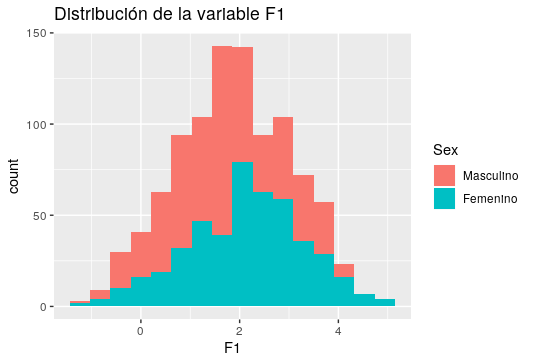
\includegraphics[scale=0.6]{dist-F1.png}  %el parámetro scale permite agrandar o chicar la imagen. En el nombre de archivo puede especificar directorios
	\caption{Histograma de la variable F1} 
	\label{fig:hist-F1}
\end{figure}

Pasamos a estudiar la normalidad de la variable. Estos son los resultados de los tests:

\begin{figure}[H]
	\centering
	\begin{subfigure}{.5\textwidth}
		\centering
		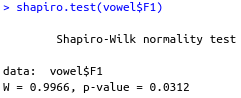
\includegraphics[width=.7\linewidth]{sw-F1.png}
		\caption{Shapiro-Wilk}
		\label{fig:sw-F1}
	\end{subfigure}%
	\begin{subfigure}{.5\textwidth}
		\centering
		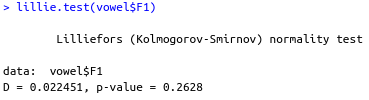
\includegraphics[width=.75\linewidth]{l-F1.png}
		\caption{Lilliefors}
		\label{fig:l-F1}
	\end{subfigure}
	\caption{Tests de normalidad sobre F1}
	\label{fig:normF1}
\end{figure}

Encontramos una discrepancia en los tests. Según el p-valor de Shapiro-Wilk, debemos rechazar la hipótesis de normalidad. Sin embargo, Lilliefors nos indica (0.2628) que no podemos rechazarla. Para esclarecer un poco más el comportamiento de F1, realizo la gráfica de densidad con una normal superpuesta con la media y desviación típica de F1:

 \begin{figure}[H] %con el [H] le obligamos a situar aquí la figura
 	\centering
 	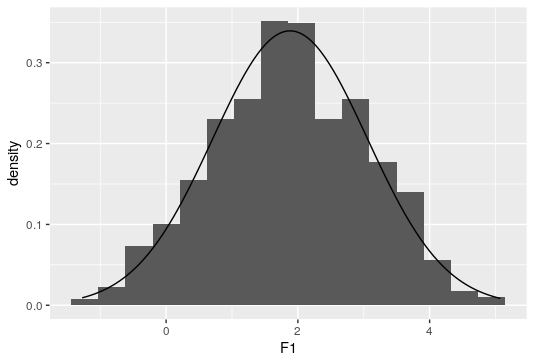
\includegraphics[scale=0.6]{density-F1.png}  %el parámetro scale permite agrandar o chicar la imagen. En el nombre de archivo puede especificar directorios
 	\caption{Histograma con la densidad de F1 y normal para comparar} 
 	\label{fig:dense-F1}
 \end{figure}

así como un QQPlot (\cite{10.1093/biomet/55.1.1}):

\begin{figure}[H] %con el [H] le obligamos a situar aquí la figura
	\centering
	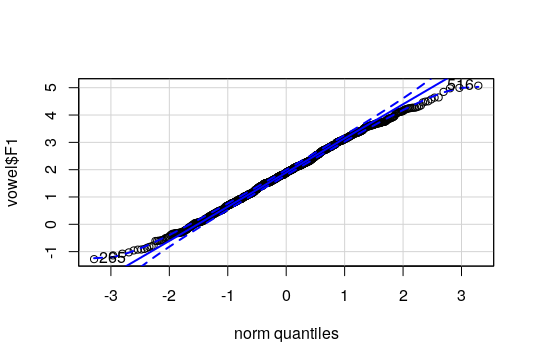
\includegraphics[scale=0.6]{qq-F1.png}  %el parámetro scale permite agrandar o chicar la imagen. En el nombre de archivo puede especificar directorios
	\caption{QQPlot de la variable F1} 
	\label{fig:qq-F1}
\end{figure}

A la luz de los resultados, podemos interpretar que F1 tiene un comportamiento muy parecido a la distribución normal. A continuación, presento los boxplots:

\begin{figure}[H]
	\centering
	\begin{subfigure}{.5\textwidth}
		\centering
		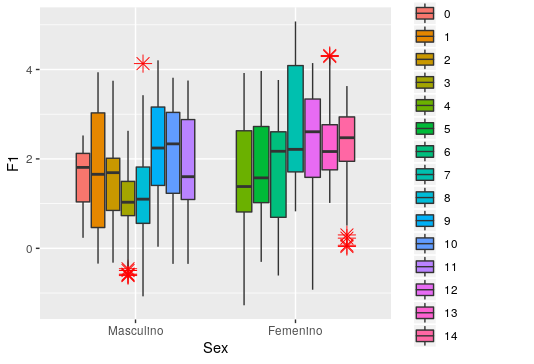
\includegraphics[width=.9\linewidth]{bps1.png}
		\caption{Por sexo}
		\label{fig:bps1}
	\end{subfigure}%
	\begin{subfigure}{.5\textwidth}
		\centering
		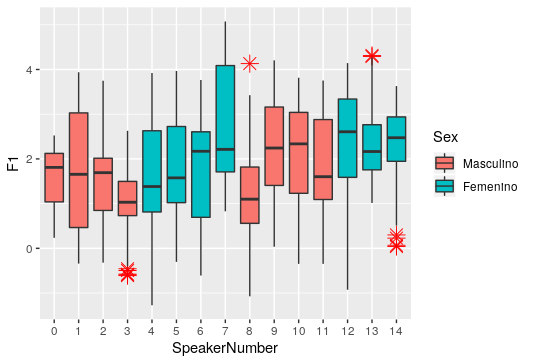
\includegraphics[width=.9\linewidth]{bpsn1.png}
		\caption{Por interlocutor}
		\label{fig:bpsn1}
	\end{subfigure}
	\caption{Boxplot para F1 estudiando sexos e interlocutores}
	\label{fig:bf1}
\end{figure}

Podemos apreciar outliers en los interlocutores 3,8,13 y 14. \\

Si ahora estudiamos los tests de normalidad por sexos, encontramos los siguientes resultados. Para los hombres

\begin{figure}[H]
	\centering
	\begin{subfigure}{.5\textwidth}
		\centering
		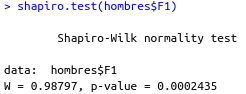
\includegraphics[width=.6\linewidth]{swh-F1.png}
		\caption{Shapiro-Wilk}
		\label{fig:swh-F1}
	\end{subfigure}%
	\begin{subfigure}{.5\textwidth}
		\centering
		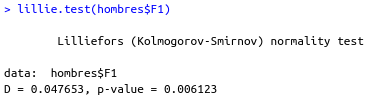
\includegraphics[width=.6\linewidth]{lh-F1.png}
		\caption{Lilliefors}
		\label{fig:lh-F1}
	\end{subfigure}
	\caption{Tests de normalidad sobre F1 (hombres)}
	\label{fig:normhF1}
\end{figure}

Ambos tests nos llevan a rechazar la hipótesis de normalidad. En el caso de las mujeres

\begin{figure}[H]
	\centering
	\begin{subfigure}{.5\textwidth}
		\centering
		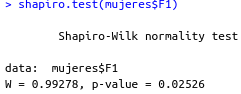
\includegraphics[width=.6\linewidth]{swm-F1.png}
		\caption{Shapiro-Wilk}
		\label{fig:swm-F1}
	\end{subfigure}%
	\begin{subfigure}{.5\textwidth}
		\centering
		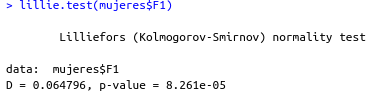
\includegraphics[width=.6\linewidth]{lm-F1.png}
		\caption{Lilliefors}
		\label{fig:lm-F1}
	\end{subfigure}
	\caption{Tests de normalidad sobre F1 (mujeres)}
	\label{fig:normmF1}
\end{figure}

también rechazamos la hipótesis nula. Por tanto, en conjunto la variable se comporta según una normal pero por separado (hombres/mujeres) no.

\subsubsection{F2}

Presentamos la variable F2. En primer lugar, reflejo un resumen estadístico de la misma así como su histograma diferenciando entre hombres y mujeres.
\begin{itemize}
	\item Media: -0.50777
	\item Mediana: -0.5725
	\item Desviación típica: 0.7119483
	\item Rango: [-2.487,-1.431]
	\item Primer y tercer cuartiles: (-0.97575,-0.06875)
	\item Asimetría: 0.2352169
	\item Curtosis: -0.1575597
\end{itemize}

Por el valor de la curtosis, la variable es platicúrtica y ligeramente asimétrica por la derecha.

\begin{figure}[H] %con el [H] le obligamos a situar aquí la figura
	\centering
	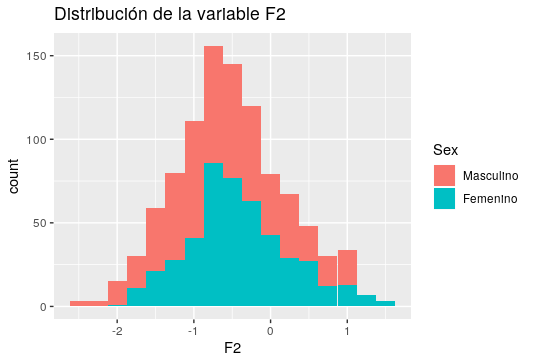
\includegraphics[scale=0.6]{dist-F2.png}  %el parámetro scale permite agrandar o chicar la imagen. En el nombre de archivo puede especificar directorios
	\caption{Histograma de la variable F2} 
	\label{fig:hist-F2}
\end{figure}


Pasamos a estudiar la normalidad de la variable. Estos son los resultados de los tests:

\begin{figure}[H]
	\centering
	\begin{subfigure}{.5\textwidth}
		\centering
		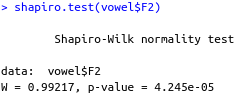
\includegraphics[width=.7\linewidth]{sw-F2.png}
		\caption{Shapiro-Wilk}
		\label{fig:sw-F2}
	\end{subfigure}%
	\begin{subfigure}{.5\textwidth}
		\centering
		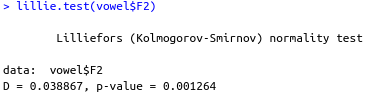
\includegraphics[width=.7\linewidth]{l-F2.png}
		\caption{Lilliefors}
		\label{fig:l-F2}
	\end{subfigure}
	\caption{Tests de normalidad sobre F2}
	\label{fig:normF2}
\end{figure}

Ambos tests nos indican que debemos rechazar la hipótesis de normalidad. En cuanto a los boxplots:

\begin{figure}[H]
	\centering
	\begin{subfigure}{.5\textwidth}
		\centering
		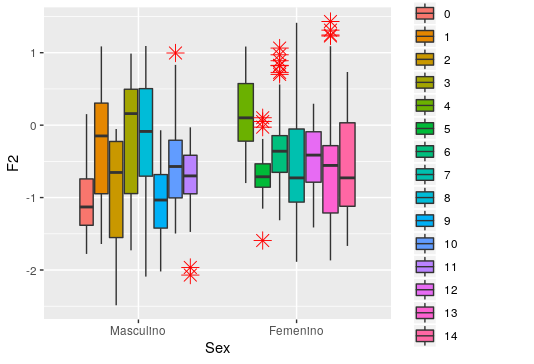
\includegraphics[width=.9\linewidth]{bps2.png}
		\caption{Por sexo}
		\label{fig:bps2}
	\end{subfigure}%
	\begin{subfigure}{.5\textwidth}
		\centering
		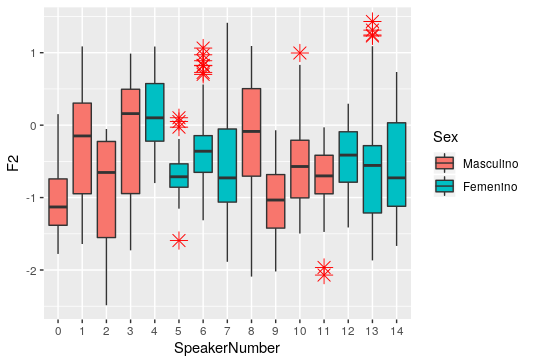
\includegraphics[width=.9\linewidth]{bpsn2.png}
		\caption{Por interlocutor}
		\label{fig:bpsn2}
	\end{subfigure}
	\caption{Boxplot para F2 estudiando sexos e interlocutores}
	\label{fig:bf2}
\end{figure}

Encontramos en F2 una gran concentración de outliers para los interlocutores 5,6,10,11 y 13. Es posible que las mediciones hayan sido erróneas. En cualquier caso, podría ser importante la aplicación de técnicas para la disminución de estos valores extraños. \\

Si ahora estudiamos los tests de normalidad por sexos, encontramos los siguientes resultados:
\begin{figure}[H]
	\centering
	\begin{subfigure}{.5\textwidth}
		\centering
		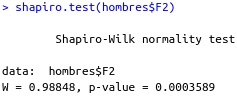
\includegraphics[width=.6\linewidth]{swh-F2.png}
		\caption{Shapiro-Wilk}
		\label{fig:swh-F2}
	\end{subfigure}%
	\begin{subfigure}{.5\textwidth}
		\centering
		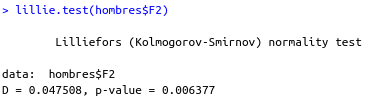
\includegraphics[width=.6\linewidth]{lh-F2.png}
		\caption{Lilliefors}
		\label{fig:lh-F2}
	\end{subfigure}
	\caption{Tests de normalidad sobre F2 (hombres)}
	\label{fig:normhF2}
\end{figure}






\begin{figure}[H]
	\centering
	\begin{subfigure}{.5\textwidth}
		\centering
		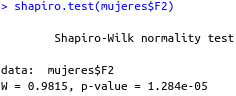
\includegraphics[width=.6\linewidth]{swm-F2.png}
		\caption{Shapiro-Wilk}
		\label{fig:swm-F2}
	\end{subfigure}%
	\begin{subfigure}{.5\textwidth}
		\centering
		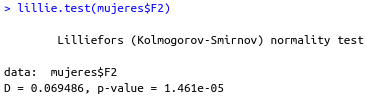
\includegraphics[width=.6\linewidth]{lm-F2.png}
		\caption{Lilliefors}
		\label{fig:lm-F2}
	\end{subfigure}
	\caption{Tests de normalidad sobre F2 (mujeres)}
	\label{fig:normmF2}
\end{figure}

Para ambos subconjuntos, los tests nos indican que debemos rechazar la hipótesis de normalidad.

\subsubsection{F3}

Como en el apartado anterior, primero reflejo un resumen estadístico de la variable:

\begin{itemize}
	\item Media: 0.5155
	\item Mediana: 0.4335
	\item Desviación típica: 0.7592613
	\item Rango: [-1.409,2.377]
	\item Primer y tercer cuartil: (-0.0655,1.096)
	\item Asimetría: 0.1287436
	\item Curtosis: -0.39925
\end{itemize}

Por el valor de la curtosis, la variable es platicúrtica y ligeramente asimétrica por la derecha.

\begin{figure}[H] %con el [H] le obligamos a situar aquí la figura
	\centering
	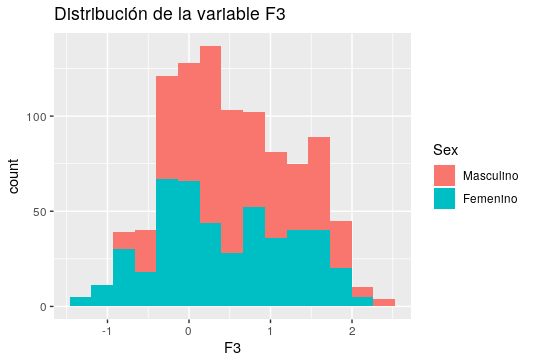
\includegraphics[scale=0.6]{dist-F3.png}  %el parámetro scale permite agrandar o chicar la imagen. En el nombre de archivo puede especificar directorios
	\caption{Histograma de la variable F3} 
	\label{fig:hist-F3}
\end{figure}

Evalúo ahora los tests de normalidad:

\begin{figure}[H]
	\centering
	\begin{subfigure}{.5\textwidth}
		\centering
		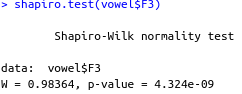
\includegraphics[width=.7\linewidth]{sw-F3.png}
		\caption{Shapiro-Wilk}
		\label{fig:sw-F3}
	\end{subfigure}%
	\begin{subfigure}{.5\textwidth}
		\centering
		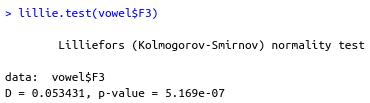
\includegraphics[width=.8\linewidth]{l-F3.png}
		\caption{Lilliefors}
		\label{fig:l-F3}
	\end{subfigure}
	\caption{Tests de normalidad sobre F3}
	\label{fig:normF3}
\end{figure}

Como se puede ver, rechazamos la hipótesis de normalidad por ser los p-valores menores de 0.05. \\

Estudiamos ahora los boxplots:

\begin{figure}[H]
	\centering
	\begin{subfigure}{.5\textwidth}
		\centering
		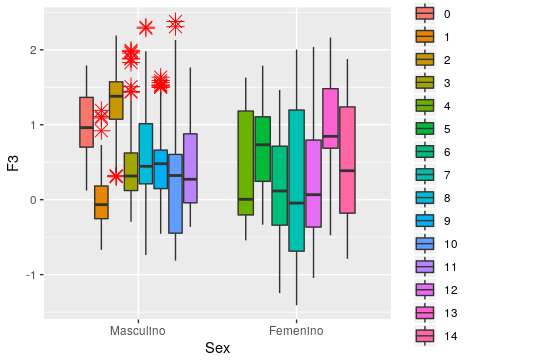
\includegraphics[width=.9\linewidth]{bps3.png}
		\caption{Por sexo}
		\label{fig:bps3}
	\end{subfigure}%
	\begin{subfigure}{.5\textwidth}
		\centering
		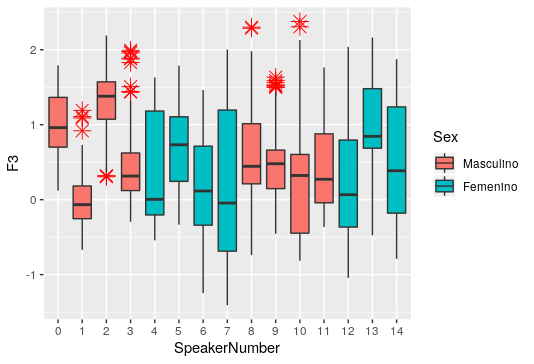
\includegraphics[width=.9\linewidth]{bpsn3.png}
		\caption{Por interlocutor}
		\label{fig:bpsn3}
	\end{subfigure}
	\caption{Boxplot para F3 estudiando sexos e interlocutores}
	\label{fig:bf3}
\end{figure}

Como se puede observar, los interlocutores 1,3 y 9 tienen bastantes outliers, mientras que los 2, 8 y 10 presentan outliers en menor medida. Con respecto a los tests de normalidad para hombres y mujeres, vemos que debemos rechazar la hipótesis de normalidad en ambos casos:

\begin{figure}[H]
	\centering
	\begin{subfigure}{.5\textwidth}
		\centering
		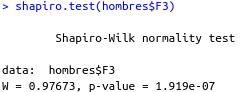
\includegraphics[width=.6\linewidth]{swh-F3.png}
		\caption{Shapiro-Wilk}
		\label{fig:swh-F3}
	\end{subfigure}%
	\begin{subfigure}{.5\textwidth}
		\centering
		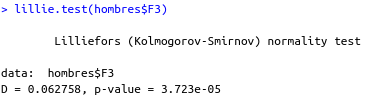
\includegraphics[width=.6\linewidth]{lh-F3.png}
		\caption{Lilliefors}
		\label{fig:lh-F3}
	\end{subfigure}
	\caption{Tests de normalidad sobre F3 (hombres)}
	\label{fig:normhF3}
\end{figure}

\begin{figure}[H]
	\centering
	\begin{subfigure}{.5\textwidth}
		\centering
		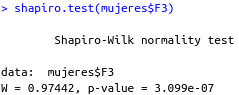
\includegraphics[width=.6\linewidth]{swm-F3.png}
		\caption{Shapiro-Wilk}
		\label{fig:swm-F3}
	\end{subfigure}%
	\begin{subfigure}{.5\textwidth}
		\centering
		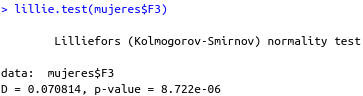
\includegraphics[width=.6\linewidth]{lm-F3.png}
		\caption{Lilliefors}
		\label{fig:lm-F3}
	\end{subfigure}
	\caption{Tests de normalidad sobre F3 (mujeres)}
	\label{fig:normmF3}
\end{figure}

\subsubsection{F4}

En primer lugar, reflejo un resumen estadístico de la variable:

\begin{itemize}
	\item Media: -0.3057
	\item Mediana: -0.299
	\item Desviación típica: 0.6646023
	\item Rango: [-2.127,1.831]
	\item Primer y tercer cuartil: (-0.769,0.1695)
	\item Asimetría: 0.01647417
	\item Curtosis: -0.2773318
\end{itemize}

Por el valor de la curtosis, la variable es platicúrtica y apenas asimétrica por la derecha. Presentamos el histograma para conocer más los datos:

\begin{figure}[H] %con el [H] le obligamos a situar aquí la figura
	\centering
	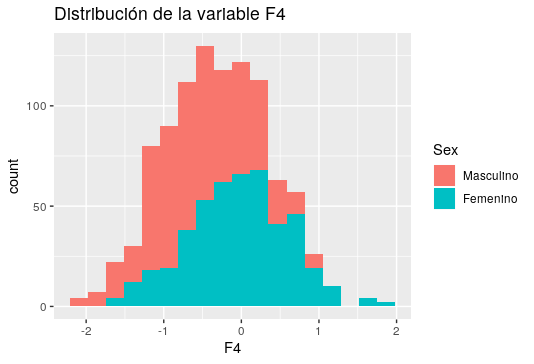
\includegraphics[scale=0.6]{dist-F4.png}  %el parámetro scale permite agrandar o chicar la imagen. En el nombre de archivo puede especificar directorios
	\caption{Histograma de la variable F4} 
	\label{fig:hist-F4}
\end{figure}

Pasamos a comprobar si F4 se distribuye según una normal. Para ello, establecemos los tests de hipótesis de Shapiro-Wilk y Lilliefors:

\begin{figure}[H]
	\centering
	\begin{subfigure}{.5\textwidth}
		\centering
		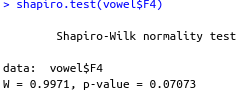
\includegraphics[width=.7\linewidth]{sw-F4.png}
		\caption{Shapiro-Wilk}
		\label{fig:sw-F4}
	\end{subfigure}%
	\begin{subfigure}{.5\textwidth}
		\centering
		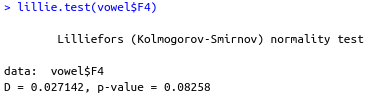
\includegraphics[width=.8\linewidth]{l-F4.png}
		\caption{Lilliefors}
		\label{fig:l-F4}
	\end{subfigure}
	\caption{Tests de normalidad sobre F4}
	\label{fig:normF4}
\end{figure}

Ambos tests indican que no podemos rechazar la hipótesis de normalidad. Confirmamos el resultado con el gráfico QQPlot.

\begin{figure}[H] %con el [H] le obligamos a situar aquí la figura
	\centering
	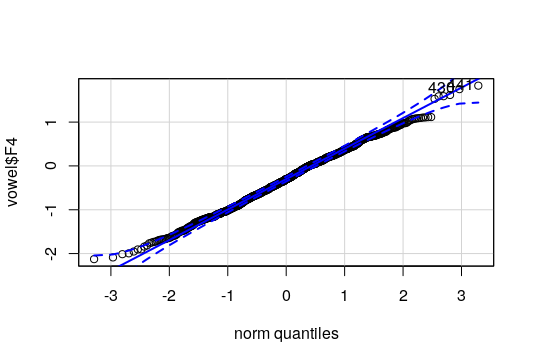
\includegraphics[scale=0.6]{qq-F4.png}  %el parámetro scale permite agrandar o chicar la imagen. En el nombre de archivo puede especificar directorios
	\caption{Gráfico QQPlot de F4} 
	\label{fig:qq-F4}
\end{figure} 

Por tanto, podemos asumir que F4 se distribuye como una normal. Estudiamos ahora los boxplots:

\begin{figure}[H]
	\centering
	\begin{subfigure}{.5\textwidth}
		\centering
		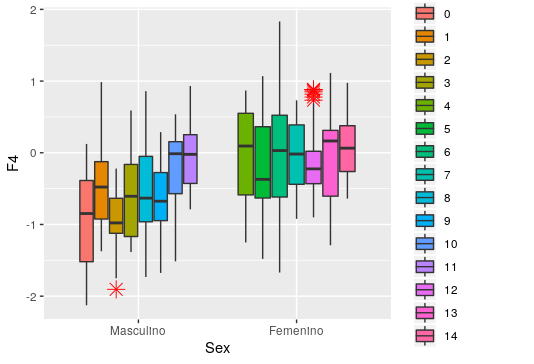
\includegraphics[width=.9\linewidth]{bps4.png}
		\caption{Por sexo}
		\label{fig:bps4}
	\end{subfigure}%
	\begin{subfigure}{.5\textwidth}
		\centering
		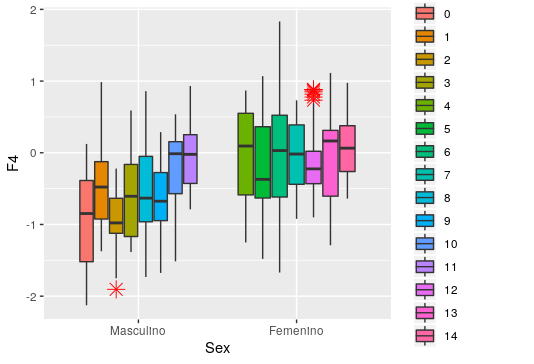
\includegraphics[width=.9\linewidth]{bpsn4.png}
		\caption{Por interlocutor}
		\label{fig:bpsn4}
	\end{subfigure}
	\caption{Boxplot para F4 estudiando sexos e interlocutores}
	\label{fig:bf4}
\end{figure}

donde apreciamos una cantidad considerable de outliers en el interlocutor 12. Además, en esta variable, las mujeres consiguen valores más altos que los hombres. \\

Por último, estudiamos los tests de normalidad por sexo. En el caso de los hombres, 

\begin{figure}[H]
	\centering
	\begin{subfigure}{.5\textwidth}
		\centering
		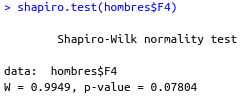
\includegraphics[width=.6\linewidth]{swh-F4.png}
		\caption{Shapiro-Wilk}
		\label{fig:swh-F4}
	\end{subfigure}%
	\begin{subfigure}{.5\textwidth}
		\centering
		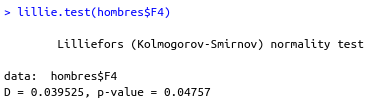
\includegraphics[width=.6\linewidth]{lh-F4.png}
		\caption{Lilliefors}
		\label{fig:lh-F4}
	\end{subfigure}
	\caption{Tests de normalidad sobre F4 (hombres)}
	\label{fig:normhF4}
\end{figure}

el test de Shapiro-Wilk indica que no podemos rechazar la hipótesis de normalidad (p valor 0.07) mientras que el de Lilliefors indica que la rechacemos. En la literatura, el test de Lilliefors resulta más fiable que el de Shapiro-Wilk por el número de instancias que tenemos, así que rechazamos la hipótesis de normalidad. \\

Para las mujeres,

\begin{figure}[H]
	\centering
	\begin{subfigure}{.5\textwidth}
		\centering
		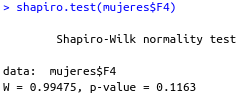
\includegraphics[width=.6\linewidth]{swm-F4.png}
		\caption{Shapiro-Wilk}
		\label{fig:swm-F4}
	\end{subfigure}%
	\begin{subfigure}{.5\textwidth}
		\centering
		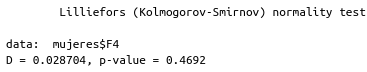
\includegraphics[width=.6\linewidth]{lm-F4.png}
		\caption{Lilliefors}
		\label{fig:lm-F4}
	\end{subfigure}
	\caption{Tests de normalidad sobre F4 (mujeres)}
	\label{fig:normmF4}
\end{figure}

los p-valores son bastante mayores que 0.05, por lo que no podemos rechazar la hipótesis de normalidad. Para confirmarlo, mostramos el QQPlot de F4 para mujeres.

\begin{figure}[H] %con el [H] le obligamos a situar aquí la figura
	\centering
	\includegraphics[scale=0.6]{qq-F4m.png}  %el parámetro scale permite agrandar o chicar la imagen. En el nombre de archivo puede especificar directorios
	\caption{Gráfico QQPlot de F4 (mujeres)} 
	\label{fig:qq-F4m}
\end{figure} 

Efectivamente, las instancias de F4 de sexo femenino siguen una distribución normal.

\subsubsection{F5}

A continuación presentamos la variable F5. Como en los casos anteriores, comenzamos por un resumen estadístico:
\begin{itemize}
	\item Media: 0.6302
	\item Mediana: 0.552
	\item Desviación típica: 0.6038711 
	\item Rango: [-0.836,2.327]
	\item Primer y tercer cuartil: (0.196,1.0285)
	\item Asimetría: 0.3559791
	\item Curtosis: -0.2964589
\end{itemize}

A la vista de los resultados, la variable es platicúrtica y ligeramente asimétrica hacia la derecha. Veamos ahora el histograma separado por sexos:

\begin{figure}[H] %con el [H] le obligamos a situar aquí la figura
	\centering
	\includegraphics[scale=0.6]{dist-F5.png}  %el parámetro scale permite agrandar o chicar la imagen. En el nombre de archivo puede especificar directorios
	\caption{Histograma de la variable F5} 
	\label{fig:hist-F5}
\end{figure}

Estudio si F5 se distribuye según una normal vía los tests estadísticos. Los resultados son los siguientes:

\begin{figure}[H]
	\centering
	\begin{subfigure}{.5\textwidth}
		\centering
		\includegraphics[width=.7\linewidth]{sw-F5.png}
		\caption{Shapiro-Wilk}
		\label{fig:sw-F5}
	\end{subfigure}%
	\begin{subfigure}{.5\textwidth}
		\centering
		\includegraphics[width=.8\linewidth]{l-F5.png}
		\caption{Lilliefors}
		\label{fig:l-F5}
	\end{subfigure}
	\caption{Tests de normalidad sobre F5}
	\label{fig:normF5}
\end{figure}

Ambos tests nos indican que debemos rechazar la hipótesis de normalidad por el bajo p-valor. Si estudiamos los boxplots, encontramos que

\begin{figure}[H]
	\centering
	\begin{subfigure}{.5\textwidth}
		\centering
		\includegraphics[width=.9\linewidth]{bps5.png}
		\caption{Por sexo}
		\label{fig:bps5}
	\end{subfigure}%
	\begin{subfigure}{.5\textwidth}
		\centering
		\includegraphics[width=.9\linewidth]{bpsn5.png}
		\caption{Por interlocutor}
		\label{fig:bpsn5}
	\end{subfigure}
	\caption{Boxplot para F5 estudiando sexos e interlocutores}
	\label{fig:bf5}
\end{figure}

con apenas outliers en los interlocutores 11 y 14. Paso a estudiar la distribución por sexos. En el caso de los hombres, comprobamos la normalidad

\begin{figure}[H]
	\centering
	\begin{subfigure}{.5\textwidth}
		\centering
		\includegraphics[width=.6\linewidth]{swh-F5.png}
		\caption{Shapiro-Wilk}
		\label{fig:swh-F5}
	\end{subfigure}%
	\begin{subfigure}{.5\textwidth}
		\centering
		\includegraphics[width=.6\linewidth]{lh-F5.png}
		\caption{Lilliefors}
		\label{fig:lh-F5}
	\end{subfigure}
	\caption{Tests de normalidad sobre F5 (hombres)}
	\label{fig:normhF5}
\end{figure}

rechazando la hipótesis de normalidad como consecuencia de los dos tests. Para las mujeres

\begin{figure}[H]
	\centering
	\begin{subfigure}{.5\textwidth}
		\centering
		\includegraphics[width=.6\linewidth]{swm-F5.png}
		\caption{Shapiro-Wilk}
		\label{fig:swm-F5}
	\end{subfigure}%
	\begin{subfigure}{.5\textwidth}
		\centering
		\includegraphics[width=.6\linewidth]{lm-F5.png}
		\caption{Lilliefors}
		\label{fig:lm-F5}
	\end{subfigure}
	\caption{Tests de normalidad sobre F5 (mujeres)}
	\label{fig:normmF5}
\end{figure}

encontramos que Shapiro-Wilk nos indica que rechacemos la hipótesis de normalidad (0.04365 < 0.05) pero Lilliefors no (0.08174>0.05). Como siempre, le doy mayor credibilidad al test de Lilliefors, por lo que no podemos rechazar la hipótesis de normalidad. Para confirmarlo, muestro el gráfico QQ.

\begin{figure}[H] %con el [H] le obligamos a situar aquí la figura
	\centering
	\includegraphics[scale=0.6]{qq-F5m.png}  %el parámetro scale permite agrandar o chicar la imagen. En el nombre de archivo puede especificar directorios
	\caption{QQPlot de la variable F5 (mujeres)} 
	\label{fig:qq-F5m}
\end{figure}

En efecto, la gráfica nos muestra que la variable se distribuye al menos de forma muy pareja a la normal. Volvemos a encontrar un caso donde el subconjunto de interlocutores masculinos difiere en distribución respecto del femenino.

\subsubsection{F6}

El resumen estadístico de la variable F6 es el siguiente:

\begin{itemize}
	\item Media: -0.004365
	\item Mediana: 0.022
	\item Desviación típica: 0.4619268
	\item Rango: [-1.537,1.403]
	\item Primer y tercer cuartiles: (-0.307,0.2965)
	\item Asimetría: -0.2055278
	\item Curtosis: 0.139262
\end{itemize}

Por lo que la variable F6 tiene una asimetría por la izquierda y es leptocúrtica. Veamos su histograma para confirmarlo.

\begin{figure}[H] %con el [H] le obligamos a situar aquí la figura
	\centering
	\includegraphics[scale=0.6]{dist-F6.png}  %el parámetro scale permite agrandar o chicar la imagen. En el nombre de archivo puede especificar directorios
	\caption{Histograma de la variable F6} 
	\label{fig:hist-F6}
\end{figure}

Examinamos si se distribuye como una normal con los tests siguientes.

\begin{figure}[H]
	\centering
	\begin{subfigure}{.5\textwidth}
		\centering
		\includegraphics[width=.7\linewidth]{sw-F6.png}
		\caption{Shapiro-Wilk}
		\label{fig:sw-F6}
	\end{subfigure}%
	\begin{subfigure}{.5\textwidth}
		\centering
		\includegraphics[width=.7\linewidth]{l-F6.png}
		\caption{Lilliefors}
		\label{fig:l-F6}
	\end{subfigure}
	\caption{Tests de normalidad sobre F6}
	\label{fig:normF6}
\end{figure}

De nuevo, Shapiro-Wilk nos indica que rechacemos la hipótesis de normalidad mientras Kolmogorov-Smirnov no nos da motivos suficientes para rechazar la hipótesis. Confirmamos que se distribuye como una normal gracias al gráfico QQ.

\begin{figure}[H] %con el [H] le obligamos a situar aquí la figura
	\centering
	\includegraphics[scale=0.6]{qq-F6.png}  %el parámetro scale permite agrandar o chicar la imagen. En el nombre de archivo puede especificar directorios
	\caption{QQPlot de la variable F6} 
	\label{fig:qq-F6}
\end{figure}

quedándose dentro de los márgenes de la normal, por lo que asumimos que F6 se distribuye como una normal. Examinemos más detenidamente su comportamiento con boxplots:

\begin{figure}[H]
	\centering
	\begin{subfigure}{.5\textwidth}
		\centering
		\includegraphics[width=.9\linewidth]{bps6.png}
		\caption{Por sexo}
		\label{fig:bps6}
	\end{subfigure}%
	\begin{subfigure}{.5\textwidth}
		\centering
		\includegraphics[width=.9\linewidth]{bpsn6.png}
		\caption{Por interlocutor}
		\label{fig:bpsn6}
	\end{subfigure}
	\caption{Boxplot para F6 estudiando sexos e interlocutores}
	\label{fig:bf6}
\end{figure}

Encontramos en ellos una gran cantidad de outliers, sobre todo concentrados en el sexo masculino (interlocutor 3 especialmente). Veamos ahora la distribución por sexos vía los tests estadísticos.

\begin{figure}[H]
	\centering
	\begin{subfigure}{.5\textwidth}
		\centering
		\includegraphics[width=.6\linewidth]{swh-F6.png}
		\caption{Shapiro-Wilk}
		\label{fig:swh-F6}
	\end{subfigure}%
	\begin{subfigure}{.5\textwidth}
		\centering
		\includegraphics[width=.6\linewidth]{lh-F6.png}
		\caption{Lilliefors}
		\label{fig:lh-F6}
	\end{subfigure}
	\caption{Tests de normalidad sobre F6 (hombres)}
	\label{fig:normhF6}
\end{figure}

El test de Shapiro-Wilk nos indica que rechacemos la hipótesis de normalidad mientras que Lilliefors, con un p-valor de 0.05132, no puede rechazar la hipótesis nula, aunque con muy poca certeza estadística. El gráfico QQ nos confirma que las colas de los datos están fuera del comportamiento de la distribución normal, por lo que el p-valor se acerca mucho a 0.05.

\begin{figure}[H] %con el [H] le obligamos a situar aquí la figura
	\centering
	\includegraphics[scale=0.6]{qq-F6h.png}  %el parámetro scale permite agrandar o chicar la imagen. En el nombre de archivo puede especificar directorios
	\caption{QQPlot de la variable F6 (hombres)} 
	\label{fig:qq-F6h}
\end{figure}

Este resultado puede venir influenciado por la gran cantidad de outliers. En el caso de las mujeres

\begin{figure}[H]
	\centering
	\begin{subfigure}{.5\textwidth}
		\centering
		\includegraphics[width=.6\linewidth]{swm-F6.png}
		\caption{Shapiro-Wilk}
		\label{fig:swm-F6}
	\end{subfigure}%
	\begin{subfigure}{.5\textwidth}
		\centering
		\includegraphics[width=.6\linewidth]{lm-F6.png}
		\caption{Lilliefors}
		\label{fig:lm-F6}
	\end{subfigure}
	\caption{Tests de normalidad sobre F6 (mujeres)}
	\label{fig:normmF6}
\end{figure}

ambos tests nos indican que no podemos rechazar la hipótesis de normalidad. Además, el gráfico QQ nos lo confirma

\begin{figure}[H] %con el [H] le obligamos a situar aquí la figura
	\centering
	\includegraphics[scale=0.6]{qq-F6m.png}  %el parámetro scale permite agrandar o chicar la imagen. En el nombre de archivo puede especificar directorios
	\caption{QQPlot de la variable F6 (mujeres)} 
	\label{fig:qq-F6m}
\end{figure}

por lo que asumimos que la variable F6 para las mujeres sigue una distribución normal.

\subsubsection{F7}

Como en todas las anteriores, presento el resumen estadístico de la variable F7 y su histograma.

\begin{itemize}
	\item Media: 0.33655
	\item Mediana: 0.328
	\item Desviación típica: 0.5733020
	\item Rango: [-1.293,2.039]
	\item Primer y tercer cuartiles: (-0.09575,0.77)
	\item Asimetría: 0.005939385
	\item Curtosis: -0.4980897
\end{itemize}


La variable apenas presenta asimetría por la derecha y es platicúrtica.

\begin{figure}[H] %con el [H] le obligamos a situar aquí la figura
	\centering
	\includegraphics[scale=0.6]{dist-F7.png}  %el parámetro scale permite agrandar o chicar la imagen. En el nombre de archivo puede especificar directorios
	\caption{Histograma de la variable F7} 
	\label{fig:hist-F7}
\end{figure}

Podemos ver, gracias al histograma, que la población de mujeres tiene gran asimetría por la derecha (0.4939301). Estudiando los tests estadísticos para la normalidad

\begin{figure}[H]
	\centering
	\begin{subfigure}{.5\textwidth}
		\centering
		\includegraphics[width=.7\linewidth]{sw-F7.png}
		\caption{Shapiro-Wilk}
		\label{fig:sw-F7}
	\end{subfigure}%
	\begin{subfigure}{.5\textwidth}
		\centering
		\includegraphics[width=.7\linewidth]{l-F7.png}
		\caption{Lilliefors}
		\label{fig:l-F7}
	\end{subfigure}
	\caption{Tests de normalidad sobre F7}
	\label{fig:normF7}
\end{figure}

vemos que ambos tests nos hacen rechazar la hipótesis de normalidad. Si observamos los boxplots

\begin{figure}[H]
	\centering
	\begin{subfigure}{.5\textwidth}
		\centering
		\includegraphics[width=.9\linewidth]{bps7.png}
		\caption{Por sexo}
		\label{fig:bps7}
	\end{subfigure}%
	\begin{subfigure}{.5\textwidth}
		\centering
		\includegraphics[width=.9\linewidth]{bpsn7.png}
		\caption{Por interlocutor}
		\label{fig:bpsn7}
	\end{subfigure}
	\caption{Boxplot para F7 estudiando sexos e interlocutores}
	\label{fig:bf7}
\end{figure}

vemos varios outliers de nuevo sobre todo en los hombres (interlocutores 2,3 y 11). Si estudiamos estos conjuntos por separado

\begin{figure}[H]
	\centering
	\begin{subfigure}{.5\textwidth}
		\centering
		\includegraphics[width=.6\linewidth]{swh-F7.png}
		\caption{Shapiro-Wilk}
		\label{fig:swh-F7}
	\end{subfigure}%
	\begin{subfigure}{.5\textwidth}
		\centering
		\includegraphics[width=.6\linewidth]{lh-F7.png}
		\caption{Lilliefors}
		\label{fig:lh-F7}
	\end{subfigure}
	\caption{Tests de normalidad sobre F7 (hombres)}
	\label{fig:normhF7}
\end{figure}

ambos estadísticos nos hacen rechazar la hipótesis de normalidad (con posibles modificaciones tras tratar los outliers), al igual que las mujeres

\begin{figure}[H]
	\centering
	\begin{subfigure}{.5\textwidth}
		\centering
		\includegraphics[width=.6\linewidth]{swm-F7.png}
		\caption{Shapiro-Wilk}
		\label{fig:swm-F7}
	\end{subfigure}%
	\begin{subfigure}{.5\textwidth}
		\centering
		\includegraphics[width=.6\linewidth]{lm-F7.png}
		\caption{Lilliefors}
		\label{fig:lm-F7}
	\end{subfigure}
	\caption{Tests de normalidad sobre F7 (mujeres)}
	\label{fig:normmF7}
\end{figure}

Debido a la asimetría, una transformación de tipo logaritmo o raíz cuadrada podría corregirse y dar lugar, además, a una distribución más parecida a la normal.

\subsubsection{F8}

He aquí el resumen estadístico e histograma de la variable F8:

\begin{itemize}
	\item Media: -0.30298
	\item Mediana: -0.3025
	\item Desviación típica: 0.5701616
	\item Rango: [-1.631,1.309]
	\item Primer y tercer cuartiles: (-0.704,0.09375)
	\item Asimetría: 0.05370663
	\item Curtosis: -0.465887
\end{itemize}


La variable presenta asimetría por la derecha y es platicúrtica.

\begin{figure}[H] %con el [H] le obligamos a situar aquí la figura
	\centering
	\includegraphics[scale=0.6]{dist-F8.png}  %el parámetro scale permite agrandar o chicar la imagen. En el nombre de archivo puede especificar directorios
	\caption{Histograma de la variable F8} 
	\label{fig:hist-F8}
\end{figure}

Estudio la distribución de F8 vía los tests estadísticos con hipótesis nula que la variable sigue una distribución normal.

\begin{figure}[H]
	\centering
	\begin{subfigure}{.5\textwidth}
		\centering
		\includegraphics[width=.7\linewidth]{sw-F8.png}
		\caption{Shapiro-Wilk}
		\label{fig:sw-F8}
	\end{subfigure}%
	\begin{subfigure}{.5\textwidth}
		\centering
		\includegraphics[width=.7\linewidth]{l-F8.png}
		\caption{Lilliefors}
		\label{fig:l-F8}
	\end{subfigure}
	\caption{Tests de normalidad sobre F8}
	\label{fig:normF8}
\end{figure}

El test de Lilliefors nos indica que no podemos rechazar la hipótesis de normalidad. Confirmamos este resultado con el gráfico QQ:

\begin{figure}[H] %con el [H] le obligamos a situar aquí la figura
	\centering
	\includegraphics[scale=0.6]{qq-F8.png}  %el parámetro scale permite agrandar o chicar la imagen. En el nombre de archivo puede especificar directorios
	\caption{QQPlot de la variable F8} 
	\label{fig:qq-F8}
\end{figure}

Si estudiamos los boxplots, vemos que la mayoría de los hombres tienen valores mayores que las mujeres. Además, encontramos ciertos outliers en los interlocutores 1,7 y 12.

\begin{figure}[H]
	\centering
	\begin{subfigure}{.5\textwidth}
		\centering
		\includegraphics[width=.9\linewidth]{bps8.png}
		\caption{Por sexo}
		\label{fig:bps8}
	\end{subfigure}%
	\begin{subfigure}{.5\textwidth}
		\centering
		\includegraphics[width=.9\linewidth]{bpsn8.png}
		\caption{Por interlocutor}
		\label{fig:bpsn8}
	\end{subfigure}
	\caption{Boxplot para F8 estudiando sexos e interlocutores}
	\label{fig:bf8}
\end{figure}

Si estudiamos ambos sexos por separado, en primer lugar los hombres,

\begin{figure}[H]
	\centering
	\begin{subfigure}{.5\textwidth}
		\centering
		\includegraphics[width=.6\linewidth]{swh-F8.png}
		\caption{Shapiro-Wilk}
		\label{fig:swh-F8}
	\end{subfigure}%
	\begin{subfigure}{.5\textwidth}
		\centering
		\includegraphics[width=.6\linewidth]{lh-F8.png}
		\caption{Lilliefors}
		\label{fig:lh-F8}
	\end{subfigure}
	\caption{Tests de normalidad sobre F8 (hombres)}
	\label{fig:normhF8}
\end{figure}

vemos que debemos rechazar la hipótesis de normalidad. Para las mujeres,

\begin{figure}[H]
	\centering
	\begin{subfigure}{.5\textwidth}
		\centering
		\includegraphics[width=.6\linewidth]{swm-F8.png}
		\caption{Shapiro-Wilk}
		\label{fig:swm-F8}
	\end{subfigure}%
	\begin{subfigure}{.5\textwidth}
		\centering
		\includegraphics[width=.6\linewidth]{lm-F8.png}
		\caption{Lilliefors}
		\label{fig:lm-F8}
	\end{subfigure}
	\caption{Tests de normalidad sobre F8 (mujeres)}
	\label{fig:normmF8}
\end{figure}

el test de Shapiro-Wilk nos invita a rechazar la hipótesis de normalidad, mientras que el de Lilliefors no encuentra suficientes motivos para rechazar la hipótesis de normalidad (p-valor > 0.05). Confirmamos ese resultado con el gráfico QQ:

\begin{figure}[H] %con el [H] le obligamos a situar aquí la figura
	\centering
	\includegraphics[scale=0.6]{qq-F8m.png}  %el parámetro scale permite agrandar o chicar la imagen. En el nombre de archivo puede especificar directorios
	\caption{QQPlot de la variable F8 (mujers)} 
	\label{fig:qq-F8m}
\end{figure}

donde vemos que la variable siempre se queda entre los márgenes establecidos para un comportamiento "normal". Vemos de nuevo una discrepancia entre el subconjunto de interlocutores masculinos y femeninos.

\subsubsection{F9}

Presentamos el resumen estadístico de la última variable, F9, junto con su histograma:

\begin{itemize}
	\item Media: -0.07134
	\item Mediana: -0.1565
	\item Desviación típica: 0.6039855
	\item Rango: [-1.68,1.396]
	\item Primer y tercer cuartiles: (-0.548,0.371)
	\item Asimetría: 0.294874
	\item Curtosis: -0.7644792
\end{itemize}

vemos que, a la luz de los resultados, existe una asimetría a la derecha de la distribución, que además es platicúrtica. Si observamos el histograma

\begin{figure}[H] %con el [H] le obligamos a situar aquí la figura
	\centering
	\includegraphics[scale=0.6]{dist-F9.png}  %el parámetro scale permite agrandar o chicar la imagen. En el nombre de archivo puede especificar directorios
	\caption{Histograma de la variable F9} 
	\label{fig:hist-F9}
\end{figure}

como se puede ver, en la distribución de hombres existe una asimetría por la derecha (0.9905848) y para las mujeres, uno por la izquierda (-0.3907809), por lo que vemos la gran disparidad entre ambas distribuciones. \\

Comprobamos ahora la normalidad de la distribución:

\begin{figure}[H]
	\centering
	\begin{subfigure}{.5\textwidth}
		\centering
		\includegraphics[width=.7\linewidth]{sw-F9.png}
		\caption{Shapiro-Wilk}
		\label{fig:sw-F9}
	\end{subfigure}%
	\begin{subfigure}{.5\textwidth}
		\centering
		\includegraphics[width=.7\linewidth]{l-F9.png}
		\caption{Lilliefors}
		\label{fig:l-F9}
	\end{subfigure}
	\caption{Tests de normalidad sobre F9}
	\label{fig:normF9}
\end{figure}

Ambos tests nos indican que debemos rechazar la hipótesis de normalidad.

Estudiamos ahora los boxplots.

\begin{figure}[H]
	\centering
	\begin{subfigure}{.5\textwidth}
		\centering
		\includegraphics[width=.9\linewidth]{bps9.png}
		\caption{Por sexo}
		\label{fig:bps9}
	\end{subfigure}%
	\begin{subfigure}{.5\textwidth}
		\centering
		\includegraphics[width=.9\linewidth]{bpsn9.png}
		\caption{Por interlocutor}
		\label{fig:bpsn9}
	\end{subfigure}
	\caption{Boxplot para F9 estudiando sexos e interlocutores}
	\label{fig:bf9}
\end{figure}

vemos apenas presencia de outliers aunque sí resultados muy dispares entre hombres y mujeres, e incluso dentro de los mismos sexos. \\


Si estudiamos la distribución de los hombres

\begin{figure}[H]
	\centering
	\begin{subfigure}{.5\textwidth}
		\centering
		\includegraphics[width=.6\linewidth]{swh-F9.png}
		\caption{Shapiro-Wilk}
		\label{fig:swh-F9}
	\end{subfigure}%
	\begin{subfigure}{.5\textwidth}
		\centering
		\includegraphics[width=.6\linewidth]{lh-F9.png}
		\caption{Lilliefors}
		\label{fig:lh-F9}
	\end{subfigure}
	\caption{Tests de normalidad sobre F9 (hombres)}
	\label{fig:normhF9}
\end{figure}

vemos que debemos rechazar la hipótesis de normalidad. Por parte de las mujeres

\begin{figure}[H]
	\centering
	\begin{subfigure}{.5\textwidth}
		\centering
		\includegraphics[width=.6\linewidth]{swm-F9.png}
		\caption{Shapiro-Wilk}
		\label{fig:swm-F9}
	\end{subfigure}%
	\begin{subfigure}{.5\textwidth}
		\centering
		\includegraphics[width=.6\linewidth]{lm-F9.png}
		\caption{Lilliefors}
		\label{fig:lm-F9}
	\end{subfigure}
	\caption{Tests de normalidad sobre F9 (mujeres)}
	\label{fig:normmF9}
\end{figure}

también rechazamos la hipótesis de normalidad.



%----------------------------------------------------------------------------------------
%	Regresión
%----------------------------------------------------------------------------------------

\section{Problema de regresión: Wankara}





%----------------------------------------------------------------------------------------
%	Clasificación
%----------------------------------------------------------------------------------------

\section{Problema de clasificación: Vowel}


\newpage
\section{Bibliografía}

%------------------------------------------------

\bibliography{citas} %archivo citas.bib que contiene las entradas 
\bibliographystyle{plain} % hay varias formas de citar

\end{document}
